\documentclass{standalone}
\usepackage{tikz}
\usetikzlibrary{patterns, positioning}

\begin{document}
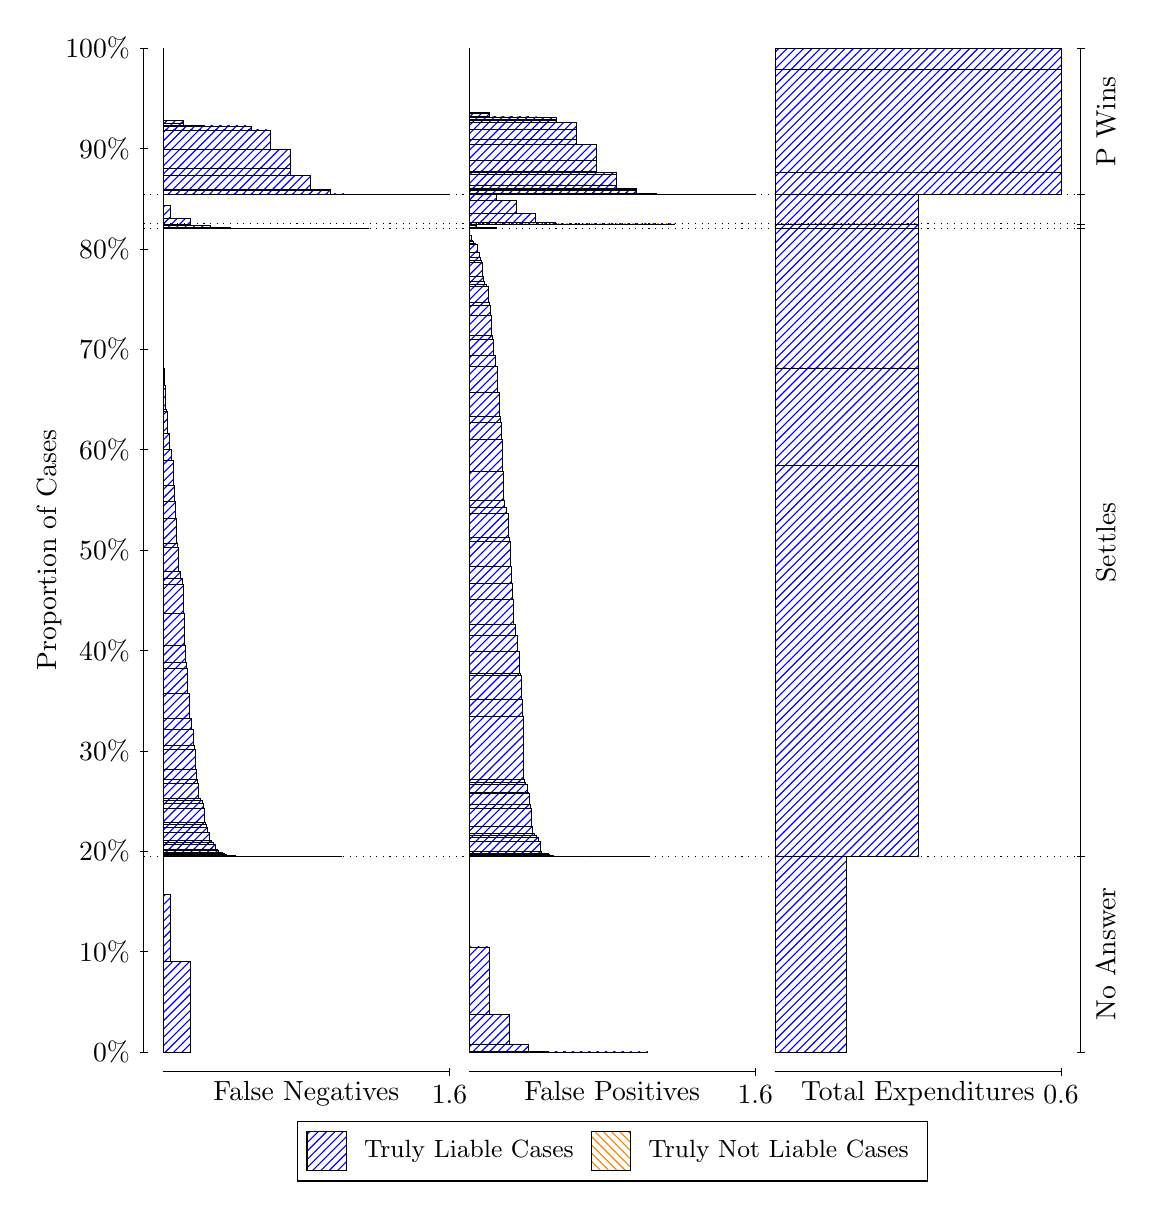
\begin{tikzpicture}
\draw[black, very thin] (1.5,1.75) -- (1.5,14.5);
\node[rotate=90, anchor=center] at (0.3, 8.125) {Proportion of Cases};
\draw[black, very thin] (1.45,1.75) -- (1.55,1.75);
\node[anchor=east] at (1.45, 1.75) {0\%};
\draw[black, very thin] (1.45,3.025) -- (1.55,3.025);
\node[anchor=east] at (1.45, 3.025) {10\%};
\draw[black, very thin] (1.45,4.3) -- (1.55,4.3);
\node[anchor=east] at (1.45, 4.3) {20\%};
\draw[black, very thin] (1.45,5.575) -- (1.55,5.575);
\node[anchor=east] at (1.45, 5.575) {30\%};
\draw[black, very thin] (1.45,6.85) -- (1.55,6.85);
\node[anchor=east] at (1.45, 6.85) {40\%};
\draw[black, very thin] (1.45,8.125) -- (1.55,8.125);
\node[anchor=east] at (1.45, 8.125) {50\%};
\draw[black, very thin] (1.45,9.4) -- (1.55,9.4);
\node[anchor=east] at (1.45, 9.4) {60\%};
\draw[black, very thin] (1.45,10.675) -- (1.55,10.675);
\node[anchor=east] at (1.45, 10.675) {70\%};
\draw[black, very thin] (1.45,11.95) -- (1.55,11.95);
\node[anchor=east] at (1.45, 11.95) {80\%};
\draw[black, very thin] (1.45,13.225) -- (1.55,13.225);
\node[anchor=east] at (1.45, 13.225) {90\%};
\draw[black, very thin] (1.45,14.5) -- (1.55,14.5);
\node[anchor=east] at (1.45, 14.5) {100\%};

\draw[black, very thin] (13.4,1.75) -- (13.4,14.5);
\draw[black, very thin] (13.35,1.75) -- (13.45,1.75);
\node[anchor=west] at (13.35, 1.75) {};
\draw[black, very thin] (13.35,4.2363) -- (13.45,4.2363);
\node[anchor=west] at (13.35, 4.2363) {};
\draw[black, very thin] (13.35,12.209) -- (13.45,12.209);
\node[anchor=west] at (13.35, 12.209) {};
\draw[black, very thin] (13.35,12.267) -- (13.45,12.267);
\node[anchor=west] at (13.35, 12.267) {};
\draw[black, very thin] (13.35,12.637) -- (13.45,12.637);
\node[anchor=west] at (13.35, 12.637) {};
\draw[black, very thin] (13.35,14.5) -- (13.45,14.5);
\node[anchor=west] at (13.35, 14.5) {};

\draw[black, very thin, pattern color=blue, pattern=north east lines] (1.75,1.75) rectangle (2.0906,2.9018);
\draw[black, very thin, pattern color=blue, pattern=north east lines] (1.75,2.9018) rectangle (1.8383,3.7553);
\draw[black, very thin, pattern color=orange, pattern=north west lines] (1.75,3.7553) rectangle (1.75,3.7553);
\draw[black, very thin, pattern color=blue, pattern=north east lines] (1.75,3.7553) rectangle (1.75,4.2363);
\draw[black, very thin, pattern color=blue, pattern=north east lines] (1.75,4.2363) rectangle (4.0208,4.2363);
\draw[black, very thin, pattern color=blue, pattern=north east lines] (1.75,4.2363) rectangle (3.9073,4.2363);
\draw[black, very thin, pattern color=blue, pattern=north east lines] (1.75,4.2363) rectangle (3.7937,4.2363);
\draw[black, very thin, pattern color=blue, pattern=north east lines] (1.75,4.2363) rectangle (3.7685,4.2363);
\draw[black, very thin, pattern color=blue, pattern=north east lines] (1.75,4.2363) rectangle (3.6802,4.2363);
\draw[black, very thin, pattern color=blue, pattern=north east lines] (1.75,4.2363) rectangle (3.655,4.2363);
\draw[black, very thin, pattern color=blue, pattern=north east lines] (1.75,4.2363) rectangle (3.5667,4.2363);
\draw[black, very thin, pattern color=blue, pattern=north east lines] (1.75,4.2363) rectangle (3.5414,4.2363);
\draw[black, very thin, pattern color=blue, pattern=north east lines] (1.75,4.2363) rectangle (3.5162,4.2363);
\draw[black, very thin, pattern color=blue, pattern=north east lines] (1.75,4.2363) rectangle (3.4531,4.2363);
\draw[black, very thin, pattern color=blue, pattern=north east lines] (1.75,4.2363) rectangle (3.4279,4.2363);
\draw[black, very thin, pattern color=blue, pattern=north east lines] (1.75,4.2363) rectangle (3.4027,4.2363);
\draw[black, very thin, pattern color=blue, pattern=north east lines] (1.75,4.2363) rectangle (3.3396,4.2363);
\draw[black, very thin, pattern color=blue, pattern=north east lines] (1.75,4.2363) rectangle (3.3144,4.2363);
\draw[black, very thin, pattern color=blue, pattern=north east lines] (1.75,4.2363) rectangle (3.2891,4.2363);
\draw[black, very thin, pattern color=blue, pattern=north east lines] (1.75,4.2363) rectangle (3.2639,4.2363);
\draw[black, very thin, pattern color=blue, pattern=north east lines] (1.75,4.2363) rectangle (3.226,4.2363);
\draw[black, very thin, pattern color=blue, pattern=north east lines] (1.75,4.2363) rectangle (3.2008,4.2363);
\draw[black, very thin, pattern color=blue, pattern=north east lines] (1.75,4.2363) rectangle (3.1756,4.2363);
\draw[black, very thin, pattern color=blue, pattern=north east lines] (1.75,4.2363) rectangle (3.1503,4.2363);
\draw[black, very thin, pattern color=blue, pattern=north east lines] (1.75,4.2363) rectangle (3.1125,4.2363);
\draw[black, very thin, pattern color=blue, pattern=north east lines] (1.75,4.2363) rectangle (3.0873,4.2363);
\draw[black, very thin, pattern color=blue, pattern=north east lines] (1.75,4.2363) rectangle (3.062,4.2363);
\draw[black, very thin, pattern color=blue, pattern=north east lines] (1.75,4.2363) rectangle (3.0368,4.2363);
\draw[black, very thin, pattern color=blue, pattern=north east lines] (1.75,4.2363) rectangle (3.0116,4.2363);
\draw[black, very thin, pattern color=blue, pattern=north east lines] (1.75,4.2363) rectangle (2.999,4.2363);
\draw[black, very thin, pattern color=blue, pattern=north east lines] (1.75,4.2363) rectangle (2.9737,4.2363);
\draw[black, very thin, pattern color=blue, pattern=north east lines] (1.75,4.2363) rectangle (2.9485,4.2363);
\draw[black, very thin, pattern color=blue, pattern=north east lines] (1.75,4.2363) rectangle (2.9233,4.2363);
\draw[black, very thin, pattern color=blue, pattern=north east lines] (1.75,4.2363) rectangle (2.898,4.2363);
\draw[black, very thin, pattern color=blue, pattern=north east lines] (1.75,4.2363) rectangle (2.8854,4.2363);
\draw[black, very thin, pattern color=blue, pattern=north east lines] (1.75,4.2363) rectangle (2.8602,4.2363);
\draw[black, very thin, pattern color=blue, pattern=north east lines] (1.75,4.2363) rectangle (2.835,4.2364);
\draw[black, very thin, pattern color=blue, pattern=north east lines] (1.75,4.2364) rectangle (2.8097,4.2364);
\draw[black, very thin, pattern color=blue, pattern=north east lines] (1.75,4.2364) rectangle (2.7845,4.2364);
\draw[black, very thin, pattern color=blue, pattern=north east lines] (1.75,4.2364) rectangle (2.7719,4.237);
\draw[black, very thin, pattern color=blue, pattern=north east lines] (1.75,4.237) rectangle (2.7593,4.237);
\draw[black, very thin, pattern color=blue, pattern=north east lines] (1.75,4.237) rectangle (2.7466,4.2371);
\draw[black, very thin, pattern color=blue, pattern=north east lines] (1.75,4.2371) rectangle (2.7214,4.2371);
\draw[black, very thin, pattern color=blue, pattern=north east lines] (1.75,4.2371) rectangle (2.6962,4.2376);
\draw[black, very thin, pattern color=blue, pattern=north east lines] (1.75,4.2376) rectangle (2.6709,4.2377);
\draw[black, very thin, pattern color=blue, pattern=north east lines] (1.75,4.2377) rectangle (2.6583,4.2429);
\draw[black, very thin, pattern color=blue, pattern=north east lines] (1.75,4.2429) rectangle (2.6457,4.2429);
\draw[black, very thin, pattern color=blue, pattern=north east lines] (1.75,4.2429) rectangle (2.6331,4.2436);
\draw[black, very thin, pattern color=blue, pattern=north east lines] (1.75,4.2436) rectangle (2.6079,4.2442);
\draw[black, very thin, pattern color=blue, pattern=north east lines] (1.75,4.2442) rectangle (2.5826,4.2494);
\draw[black, very thin, pattern color=blue, pattern=north east lines] (1.75,4.2494) rectangle (2.5574,4.2521);
\draw[black, very thin, pattern color=blue, pattern=north east lines] (1.75,4.2521) rectangle (2.5448,4.2561);
\draw[black, very thin, pattern color=blue, pattern=north east lines] (1.75,4.2561) rectangle (2.5322,4.2569);
\draw[black, very thin, pattern color=blue, pattern=north east lines] (1.75,4.2569) rectangle (2.5196,4.2744);
\draw[black, very thin, pattern color=blue, pattern=north east lines] (1.75,4.2744) rectangle (2.5069,4.2771);
\draw[black, very thin, pattern color=blue, pattern=north east lines] (1.75,4.2771) rectangle (2.4943,4.2805);
\draw[black, very thin, pattern color=blue, pattern=north east lines] (1.75,4.2805) rectangle (2.4691,4.2824);
\draw[black, very thin, pattern color=blue, pattern=north east lines] (1.75,4.2824) rectangle (2.4439,4.3059);
\draw[black, very thin, pattern color=blue, pattern=north east lines] (1.75,4.3059) rectangle (2.4312,4.3184);
\draw[black, very thin, pattern color=blue, pattern=north east lines] (1.75,4.3184) rectangle (2.4186,4.328);
\draw[black, very thin, pattern color=blue, pattern=north east lines] (1.75,4.328) rectangle (2.406,4.3911);
\draw[black, very thin, pattern color=blue, pattern=north east lines] (1.75,4.3911) rectangle (2.3934,4.3941);
\draw[black, very thin, pattern color=blue, pattern=north east lines] (1.75,4.3941) rectangle (2.3808,4.4192);
\draw[black, very thin, pattern color=blue, pattern=north east lines] (1.75,4.4192) rectangle (2.3556,4.4418);
\draw[black, very thin, pattern color=blue, pattern=north east lines] (1.75,4.4418) rectangle (2.3303,4.538);
\draw[black, very thin, pattern color=blue, pattern=north east lines] (1.75,4.538) rectangle (2.3051,4.6049);
\draw[black, very thin, pattern color=blue, pattern=north east lines] (1.75,4.6049) rectangle (2.2925,4.6396);
\draw[black, very thin, pattern color=blue, pattern=north east lines] (1.75,4.6396) rectangle (2.2799,4.671);
\draw[black, very thin, pattern color=blue, pattern=north east lines] (1.75,4.671) rectangle (2.2672,4.8393);
\draw[black, very thin, pattern color=blue, pattern=north east lines] (1.75,4.8393) rectangle (2.2546,4.9024);
\draw[black, very thin, pattern color=blue, pattern=north east lines] (1.75,4.9024) rectangle (2.242,4.9421);
\draw[black, very thin, pattern color=blue, pattern=north east lines] (1.75,4.9421) rectangle (2.2168,4.9738);
\draw[black, very thin, pattern color=blue, pattern=north east lines] (1.75,4.9738) rectangle (2.1916,5.1682);
\draw[black, very thin, pattern color=blue, pattern=north east lines] (1.75,5.1682) rectangle (2.1789,5.2166);
\draw[black, very thin, pattern color=blue, pattern=north east lines] (1.75,5.2166) rectangle (2.1663,5.3442);
\draw[black, very thin, pattern color=blue, pattern=north east lines] (1.75,5.3442) rectangle (2.1537,5.5908);
\draw[black, very thin, pattern color=blue, pattern=north east lines] (1.75,5.5908) rectangle (2.1411,5.6457);
\draw[black, very thin, pattern color=blue, pattern=north east lines] (1.75,5.6457) rectangle (2.1285,5.8478);
\draw[black, very thin, pattern color=blue, pattern=north east lines] (1.75,5.8478) rectangle (2.1032,5.987);
\draw[black, very thin, pattern color=blue, pattern=north east lines] (1.75,5.987) rectangle (2.078,6.3112);
\draw[black, very thin, pattern color=blue, pattern=north east lines] (1.75,6.3112) rectangle (2.0528,6.6219);
\draw[black, very thin, pattern color=blue, pattern=north east lines] (1.75,6.6219) rectangle (2.0402,6.6987);
\draw[black, very thin, pattern color=blue, pattern=north east lines] (1.75,6.6987) rectangle (2.0275,6.9177);
\draw[black, very thin, pattern color=blue, pattern=north east lines] (1.75,6.9177) rectangle (2.0149,7.318);
\draw[black, very thin, pattern color=blue, pattern=north east lines] (1.75,7.318) rectangle (2.0023,7.6855);
\draw[black, very thin, pattern color=blue, pattern=north east lines] (1.75,7.6855) rectangle (1.9897,7.7716);
\draw[black, very thin, pattern color=blue, pattern=north east lines] (1.75,7.7716) rectangle (1.9645,7.8511);
\draw[black, very thin, pattern color=blue, pattern=north east lines] (1.75,7.8511) rectangle (1.9392,8.1613);
\draw[black, very thin, pattern color=blue, pattern=north east lines] (1.75,8.1613) rectangle (1.9266,8.2154);
\draw[black, very thin, pattern color=blue, pattern=north east lines] (1.75,8.2154) rectangle (1.914,8.5227);
\draw[black, very thin, pattern color=blue, pattern=north east lines] (1.75,8.5227) rectangle (1.9014,8.7444);
\draw[black, very thin, pattern color=blue, pattern=north east lines] (1.75,8.7444) rectangle (1.8888,8.9482);
\draw[black, very thin, pattern color=blue, pattern=north east lines] (1.75,8.9482) rectangle (1.8762,9.2626);
\draw[black, very thin, pattern color=blue, pattern=north east lines] (1.75,9.2626) rectangle (1.8509,9.4005);
\draw[black, very thin, pattern color=blue, pattern=north east lines] (1.75,9.4005) rectangle (1.8257,9.6123);
\draw[black, very thin, pattern color=blue, pattern=north east lines] (1.75,9.6123) rectangle (1.8005,9.8812);
\draw[black, very thin, pattern color=blue, pattern=north east lines] (1.75,9.8812) rectangle (1.7878,9.9115);
\draw[black, very thin, pattern color=blue, pattern=north east lines] (1.75,9.9115) rectangle (1.7752,10.211);
\draw[black, very thin, pattern color=blue, pattern=north east lines] (1.75,10.211) rectangle (1.7626,10.428);
\draw[black, very thin, pattern color=orange, pattern=north west lines] (1.75,10.428) rectangle (1.75,10.428);
\draw[black, very thin, pattern color=blue, pattern=north east lines] (1.75,10.428) rectangle (1.75,12.209);
\draw[black, very thin, pattern color=blue, pattern=north east lines] (1.75,12.209) rectangle (4.3615,12.209);
\draw[black, very thin, pattern color=blue, pattern=north east lines] (1.75,12.209) rectangle (4.1091,12.209);
\draw[black, very thin, pattern color=blue, pattern=north east lines] (1.75,12.209) rectangle (3.8568,12.209);
\draw[black, very thin, pattern color=blue, pattern=north east lines] (1.75,12.209) rectangle (3.6045,12.209);
\draw[black, very thin, pattern color=blue, pattern=north east lines] (1.75,12.209) rectangle (3.3522,12.209);
\draw[black, very thin, pattern color=blue, pattern=north east lines] (1.75,12.209) rectangle (3.0999,12.209);
\draw[black, very thin, pattern color=blue, pattern=north east lines] (1.75,12.209) rectangle (2.8476,12.21);
\draw[black, very thin, pattern color=blue, pattern=north east lines] (1.75,12.21) rectangle (2.5953,12.225);
\draw[black, very thin, pattern color=blue, pattern=north east lines] (1.75,12.225) rectangle (2.3429,12.252);
\draw[black, very thin, pattern color=blue, pattern=north east lines] (1.75,12.252) rectangle (2.0906,12.267);
\draw[black, very thin, pattern color=orange, pattern=north west lines] (1.75,12.267) rectangle (1.75,12.267);
\draw[black, very thin, pattern color=blue, pattern=north east lines] (1.75,12.267) rectangle (2.0906,12.341);
\draw[black, very thin, pattern color=blue, pattern=north east lines] (1.75,12.341) rectangle (1.8383,12.5);
\draw[black, very thin, pattern color=orange, pattern=north west lines] (1.75,12.5) rectangle (1.75,12.5);
\draw[black, very thin, pattern color=blue, pattern=north east lines] (1.75,12.5) rectangle (1.75,12.637);
\draw[black, very thin, pattern color=blue, pattern=north east lines] (1.75,12.637) rectangle (5.3833,12.637);
\draw[black, very thin, pattern color=blue, pattern=north east lines] (1.75,12.637) rectangle (5.131,12.637);
\draw[black, very thin, pattern color=blue, pattern=north east lines] (1.75,12.637) rectangle (4.8787,12.637);
\draw[black, very thin, pattern color=blue, pattern=north east lines] (1.75,12.637) rectangle (4.6264,12.638);
\draw[black, very thin, pattern color=blue, pattern=north east lines] (1.75,12.638) rectangle (4.3741,12.639);
\draw[black, very thin, pattern color=blue, pattern=north east lines] (1.75,12.639) rectangle (4.1218,12.643);
\draw[black, very thin, pattern color=blue, pattern=north east lines] (1.75,12.643) rectangle (4.1218,12.649);
\draw[black, very thin, pattern color=blue, pattern=north east lines] (1.75,12.649) rectangle (3.8694,12.699);
\draw[black, very thin, pattern color=blue, pattern=north east lines] (1.75,12.699) rectangle (3.8694,12.704);
\draw[black, very thin, pattern color=blue, pattern=north east lines] (1.75,12.704) rectangle (3.6171,12.884);
\draw[black, very thin, pattern color=blue, pattern=north east lines] (1.75,12.884) rectangle (3.5162,12.884);
\draw[black, very thin, pattern color=blue, pattern=north east lines] (1.75,12.884) rectangle (3.3648,12.979);
\draw[black, very thin, pattern color=blue, pattern=north east lines] (1.75,12.979) rectangle (3.3648,13.214);
\draw[black, very thin, pattern color=blue, pattern=north east lines] (1.75,13.214) rectangle (3.2639,13.214);
\draw[black, very thin, pattern color=blue, pattern=north east lines] (1.75,13.214) rectangle (3.2639,13.214);
\draw[black, very thin, pattern color=blue, pattern=north east lines] (1.75,13.214) rectangle (3.1125,13.459);
\draw[black, very thin, pattern color=blue, pattern=north east lines] (1.75,13.459) rectangle (3.0116,13.459);
\draw[black, very thin, pattern color=blue, pattern=north east lines] (1.75,13.459) rectangle (2.8602,13.46);
\draw[black, very thin, pattern color=blue, pattern=north east lines] (1.75,13.46) rectangle (2.8602,13.51);
\draw[black, very thin, pattern color=blue, pattern=north east lines] (1.75,13.51) rectangle (2.8602,13.511);
\draw[black, very thin, pattern color=blue, pattern=north east lines] (1.75,13.511) rectangle (2.7593,13.511);
\draw[black, very thin, pattern color=blue, pattern=north east lines] (1.75,13.511) rectangle (2.7593,13.511);
\draw[black, very thin, pattern color=blue, pattern=north east lines] (1.75,13.511) rectangle (2.6079,13.512);
\draw[black, very thin, pattern color=blue, pattern=north east lines] (1.75,13.512) rectangle (2.6079,13.512);
\draw[black, very thin, pattern color=blue, pattern=north east lines] (1.75,13.512) rectangle (2.5069,13.512);
\draw[black, very thin, pattern color=blue, pattern=north east lines] (1.75,13.512) rectangle (2.5069,13.512);
\draw[black, very thin, pattern color=blue, pattern=north east lines] (1.75,13.512) rectangle (2.5069,13.512);
\draw[black, very thin, pattern color=blue, pattern=north east lines] (1.75,13.512) rectangle (2.3556,13.512);
\draw[black, very thin, pattern color=blue, pattern=north east lines] (1.75,13.512) rectangle (2.3556,13.512);
\draw[black, very thin, pattern color=blue, pattern=north east lines] (1.75,13.512) rectangle (2.2546,13.512);
\draw[black, very thin, pattern color=blue, pattern=north east lines] (1.75,13.512) rectangle (2.2546,13.516);
\draw[black, very thin, pattern color=blue, pattern=north east lines] (1.75,13.516) rectangle (2.1032,13.516);
\draw[black, very thin, pattern color=blue, pattern=north east lines] (1.75,13.516) rectangle (2.1032,13.516);
\draw[black, very thin, pattern color=blue, pattern=north east lines] (1.75,13.516) rectangle (2.0023,13.541);
\draw[black, very thin, pattern color=blue, pattern=north east lines] (1.75,13.541) rectangle (2.0023,13.55);
\draw[black, very thin, pattern color=blue, pattern=north east lines] (1.75,13.55) rectangle (2.0023,13.584);
\draw[black, very thin, pattern color=blue, pattern=north east lines] (1.75,13.584) rectangle (1.8509,13.584);
\draw[black, very thin, pattern color=blue, pattern=north east lines] (1.75,13.584) rectangle (1.8509,13.584);
\draw[black, very thin, pattern color=orange, pattern=north west lines] (1.75,13.584) rectangle (1.75,13.584);
\draw[black, very thin, pattern color=blue, pattern=north east lines] (1.75,13.584) rectangle (1.75,14.5);
\draw[black, very thin, pattern color=orange, pattern=north west lines] (5.6333,1.75) rectangle (7.9042,1.75);
\draw[black, very thin, pattern color=blue, pattern=north east lines] (5.6333,1.75) rectangle (7.9042,1.75);
\draw[black, very thin, pattern color=blue, pattern=north east lines] (5.6333,1.75) rectangle (7.6519,1.75);
\draw[black, very thin, pattern color=blue, pattern=north east lines] (5.6333,1.75) rectangle (7.3995,1.75);
\draw[black, very thin, pattern color=blue, pattern=north east lines] (5.6333,1.75) rectangle (7.1472,1.75);
\draw[black, very thin, pattern color=blue, pattern=north east lines] (5.6333,1.75) rectangle (6.8949,1.7503);
\draw[black, very thin, pattern color=blue, pattern=north east lines] (5.6333,1.7503) rectangle (6.6426,1.7582);
\draw[black, very thin, pattern color=blue, pattern=north east lines] (5.6333,1.7582) rectangle (6.3903,1.8431);
\draw[black, very thin, pattern color=blue, pattern=north east lines] (5.6333,1.8431) rectangle (6.138,2.231);
\draw[black, very thin, pattern color=blue, pattern=north east lines] (5.6333,2.231) rectangle (5.8856,3.0845);
\draw[black, very thin, pattern color=blue, pattern=north east lines] (5.6333,3.0845) rectangle (5.6333,4.2363);
\draw[black, very thin, pattern color=orange, pattern=north west lines] (5.6333,4.2363) rectangle (7.9042,4.2363);
\draw[black, very thin, pattern color=blue, pattern=north east lines] (5.6333,4.2363) rectangle (7.9042,4.2363);
\draw[black, very thin, pattern color=orange, pattern=north west lines] (5.6333,4.2363) rectangle (7.7906,4.2363);
\draw[black, very thin, pattern color=blue, pattern=north east lines] (5.6333,4.2363) rectangle (7.7906,4.2363);
\draw[black, very thin, pattern color=orange, pattern=north west lines] (5.6333,4.2363) rectangle (7.6771,4.2363);
\draw[black, very thin, pattern color=blue, pattern=north east lines] (5.6333,4.2363) rectangle (7.6771,4.2363);
\draw[black, very thin, pattern color=blue, pattern=north east lines] (5.6333,4.2363) rectangle (7.6519,4.2363);
\draw[black, very thin, pattern color=orange, pattern=north west lines] (5.6333,4.2363) rectangle (7.5635,4.2363);
\draw[black, very thin, pattern color=blue, pattern=north east lines] (5.6333,4.2363) rectangle (7.5635,4.2363);
\draw[black, very thin, pattern color=blue, pattern=north east lines] (5.6333,4.2363) rectangle (7.5383,4.2363);
\draw[black, very thin, pattern color=orange, pattern=north west lines] (5.6333,4.2363) rectangle (7.45,4.2363);
\draw[black, very thin, pattern color=blue, pattern=north east lines] (5.6333,4.2363) rectangle (7.45,4.2363);
\draw[black, very thin, pattern color=blue, pattern=north east lines] (5.6333,4.2363) rectangle (7.4248,4.2363);
\draw[black, very thin, pattern color=blue, pattern=north east lines] (5.6333,4.2363) rectangle (7.3995,4.2363);
\draw[black, very thin, pattern color=orange, pattern=north west lines] (5.6333,4.2363) rectangle (7.3365,4.2363);
\draw[black, very thin, pattern color=blue, pattern=north east lines] (5.6333,4.2363) rectangle (7.3365,4.2363);
\draw[black, very thin, pattern color=blue, pattern=north east lines] (5.6333,4.2363) rectangle (7.3112,4.2363);
\draw[black, very thin, pattern color=blue, pattern=north east lines] (5.6333,4.2363) rectangle (7.286,4.2363);
\draw[black, very thin, pattern color=orange, pattern=north west lines] (5.6333,4.2363) rectangle (7.2229,4.2363);
\draw[black, very thin, pattern color=blue, pattern=north east lines] (5.6333,4.2363) rectangle (7.2229,4.2363);
\draw[black, very thin, pattern color=blue, pattern=north east lines] (5.6333,4.2363) rectangle (7.1977,4.2363);
\draw[black, very thin, pattern color=blue, pattern=north east lines] (5.6333,4.2363) rectangle (7.1725,4.2363);
\draw[black, very thin, pattern color=blue, pattern=north east lines] (5.6333,4.2363) rectangle (7.1472,4.2363);
\draw[black, very thin, pattern color=orange, pattern=north west lines] (5.6333,4.2363) rectangle (7.1094,4.2363);
\draw[black, very thin, pattern color=blue, pattern=north east lines] (5.6333,4.2363) rectangle (7.1094,4.2363);
\draw[black, very thin, pattern color=blue, pattern=north east lines] (5.6333,4.2363) rectangle (7.0841,4.2363);
\draw[black, very thin, pattern color=blue, pattern=north east lines] (5.6333,4.2363) rectangle (7.0589,4.2363);
\draw[black, very thin, pattern color=blue, pattern=north east lines] (5.6333,4.2363) rectangle (7.0337,4.2363);
\draw[black, very thin, pattern color=orange, pattern=north west lines] (5.6333,4.2363) rectangle (6.9958,4.2363);
\draw[black, very thin, pattern color=blue, pattern=north east lines] (5.6333,4.2363) rectangle (6.9958,4.2363);
\draw[black, very thin, pattern color=blue, pattern=north east lines] (5.6333,4.2363) rectangle (6.9706,4.2363);
\draw[black, very thin, pattern color=blue, pattern=north east lines] (5.6333,4.2363) rectangle (6.9454,4.2364);
\draw[black, very thin, pattern color=blue, pattern=north east lines] (5.6333,4.2364) rectangle (6.9201,4.2364);
\draw[black, very thin, pattern color=blue, pattern=north east lines] (5.6333,4.2364) rectangle (6.8949,4.2364);
\draw[black, very thin, pattern color=orange, pattern=north west lines] (5.6333,4.2364) rectangle (6.8823,4.2364);
\draw[black, very thin, pattern color=blue, pattern=north east lines] (5.6333,4.2364) rectangle (6.8823,4.2365);
\draw[black, very thin, pattern color=blue, pattern=north east lines] (5.6333,4.2365) rectangle (6.8571,4.2365);
\draw[black, very thin, pattern color=blue, pattern=north east lines] (5.6333,4.2365) rectangle (6.8318,4.2365);
\draw[black, very thin, pattern color=blue, pattern=north east lines] (5.6333,4.2365) rectangle (6.8066,4.237);
\draw[black, very thin, pattern color=blue, pattern=north east lines] (5.6333,4.237) rectangle (6.7814,4.2371);
\draw[black, very thin, pattern color=orange, pattern=north west lines] (5.6333,4.2371) rectangle (6.7687,4.2371);
\draw[black, very thin, pattern color=blue, pattern=north east lines] (5.6333,4.2371) rectangle (6.7687,4.239);
\draw[black, very thin, pattern color=blue, pattern=north east lines] (5.6333,4.239) rectangle (6.7435,4.2397);
\draw[black, very thin, pattern color=blue, pattern=north east lines] (5.6333,4.2397) rectangle (6.7183,4.2402);
\draw[black, very thin, pattern color=blue, pattern=north east lines] (5.6333,4.2402) rectangle (6.6931,4.2454);
\draw[black, very thin, pattern color=blue, pattern=north east lines] (5.6333,4.2454) rectangle (6.6678,4.247);
\draw[black, very thin, pattern color=orange, pattern=north west lines] (5.6333,4.247) rectangle (6.6552,4.247);
\draw[black, very thin, pattern color=blue, pattern=north east lines] (5.6333,4.247) rectangle (6.6552,4.2671);
\draw[black, very thin, pattern color=blue, pattern=north east lines] (5.6333,4.2671) rectangle (6.6426,4.2677);
\draw[black, very thin, pattern color=blue, pattern=north east lines] (5.6333,4.2677) rectangle (6.63,4.2738);
\draw[black, very thin, pattern color=blue, pattern=north east lines] (5.6333,4.2738) rectangle (6.6047,4.2758);
\draw[black, very thin, pattern color=blue, pattern=north east lines] (5.6333,4.2758) rectangle (6.5795,4.2777);
\draw[black, very thin, pattern color=blue, pattern=north east lines] (5.6333,4.2777) rectangle (6.5543,4.3022);
\draw[black, very thin, pattern color=orange, pattern=north west lines] (5.6333,4.3022) rectangle (6.5417,4.3022);
\draw[black, very thin, pattern color=blue, pattern=north east lines] (5.6333,4.3022) rectangle (6.5417,4.4259);
\draw[black, very thin, pattern color=blue, pattern=north east lines] (5.6333,4.4259) rectangle (6.5291,4.4278);
\draw[black, very thin, pattern color=blue, pattern=north east lines] (5.6333,4.4278) rectangle (6.5164,4.4728);
\draw[black, very thin, pattern color=blue, pattern=north east lines] (5.6333,4.4728) rectangle (6.4912,4.4995);
\draw[black, very thin, pattern color=blue, pattern=north east lines] (5.6333,4.4995) rectangle (6.466,4.5212);
\draw[black, very thin, pattern color=blue, pattern=north east lines] (5.6333,4.5212) rectangle (6.4407,4.6159);
\draw[black, very thin, pattern color=orange, pattern=north west lines] (5.6333,4.6159) rectangle (6.4281,4.6159);
\draw[black, very thin, pattern color=blue, pattern=north east lines] (5.6333,4.6159) rectangle (6.4281,4.8502);
\draw[black, very thin, pattern color=blue, pattern=north east lines] (5.6333,4.8502) rectangle (6.4155,4.8914);
\draw[black, very thin, pattern color=blue, pattern=north east lines] (5.6333,4.8914) rectangle (6.4029,5.0379);
\draw[black, very thin, pattern color=blue, pattern=north east lines] (5.6333,5.0379) rectangle (6.3903,5.0508);
\draw[black, very thin, pattern color=blue, pattern=north east lines] (5.6333,5.0508) rectangle (6.3777,5.1475);
\draw[black, very thin, pattern color=blue, pattern=north east lines] (5.6333,5.1475) rectangle (6.3524,5.179);
\draw[black, very thin, pattern color=blue, pattern=north east lines] (5.6333,5.179) rectangle (6.3272,5.2109);
\draw[black, very thin, pattern color=orange, pattern=north west lines] (5.6333,5.2109) rectangle (6.3146,5.2109);
\draw[black, very thin, pattern color=blue, pattern=north east lines] (5.6333,5.2109) rectangle (6.3146,6.0171);
\draw[black, very thin, pattern color=blue, pattern=north east lines] (5.6333,6.0171) rectangle (6.302,6.2335);
\draw[black, very thin, pattern color=blue, pattern=north east lines] (5.6333,6.2335) rectangle (6.2894,6.5335);
\draw[black, very thin, pattern color=blue, pattern=north east lines] (5.6333,6.5335) rectangle (6.2767,6.5637);
\draw[black, very thin, pattern color=blue, pattern=north east lines] (5.6333,6.5637) rectangle (6.2641,6.8327);
\draw[black, very thin, pattern color=blue, pattern=north east lines] (5.6333,6.8327) rectangle (6.2389,7.0445);
\draw[black, very thin, pattern color=blue, pattern=north east lines] (5.6333,7.0445) rectangle (6.2137,7.1823);
\draw[black, very thin, pattern color=blue, pattern=north east lines] (5.6333,7.1823) rectangle (6.1884,7.4967);
\draw[black, very thin, pattern color=blue, pattern=north east lines] (5.6333,7.4967) rectangle (6.1758,7.7005);
\draw[black, very thin, pattern color=blue, pattern=north east lines] (5.6333,7.7005) rectangle (6.1632,7.9222);
\draw[black, very thin, pattern color=blue, pattern=north east lines] (5.6333,7.9222) rectangle (6.1506,8.2295);
\draw[black, very thin, pattern color=blue, pattern=north east lines] (5.6333,8.2295) rectangle (6.138,8.2836);
\draw[black, very thin, pattern color=blue, pattern=north east lines] (5.6333,8.2836) rectangle (6.1253,8.5939);
\draw[black, very thin, pattern color=blue, pattern=north east lines] (5.6333,8.5939) rectangle (6.1001,8.6733);
\draw[black, very thin, pattern color=blue, pattern=north east lines] (5.6333,8.6733) rectangle (6.0749,8.7594);
\draw[black, very thin, pattern color=blue, pattern=north east lines] (5.6333,8.7594) rectangle (6.0623,9.1269);
\draw[black, very thin, pattern color=blue, pattern=north east lines] (5.6333,9.1269) rectangle (6.0497,9.5272);
\draw[black, very thin, pattern color=blue, pattern=north east lines] (5.6333,9.5272) rectangle (6.037,9.7462);
\draw[black, very thin, pattern color=blue, pattern=north east lines] (5.6333,9.7462) rectangle (6.0244,9.823);
\draw[black, very thin, pattern color=blue, pattern=north east lines] (5.6333,9.823) rectangle (6.0118,10.134);
\draw[black, very thin, pattern color=blue, pattern=north east lines] (5.6333,10.134) rectangle (5.9866,10.458);
\draw[black, very thin, pattern color=blue, pattern=north east lines] (5.6333,10.458) rectangle (5.9613,10.597);
\draw[black, very thin, pattern color=blue, pattern=north east lines] (5.6333,10.597) rectangle (5.9361,10.799);
\draw[black, very thin, pattern color=blue, pattern=north east lines] (5.6333,10.799) rectangle (5.9235,10.854);
\draw[black, very thin, pattern color=blue, pattern=north east lines] (5.6333,10.854) rectangle (5.9109,11.101);
\draw[black, very thin, pattern color=blue, pattern=north east lines] (5.6333,11.101) rectangle (5.8983,11.228);
\draw[black, very thin, pattern color=blue, pattern=north east lines] (5.6333,11.228) rectangle (5.8856,11.277);
\draw[black, very thin, pattern color=blue, pattern=north east lines] (5.6333,11.277) rectangle (5.873,11.471);
\draw[black, very thin, pattern color=blue, pattern=north east lines] (5.6333,11.471) rectangle (5.8478,11.503);
\draw[black, very thin, pattern color=blue, pattern=north east lines] (5.6333,11.503) rectangle (5.8226,11.543);
\draw[black, very thin, pattern color=blue, pattern=north east lines] (5.6333,11.543) rectangle (5.81,11.606);
\draw[black, very thin, pattern color=blue, pattern=north east lines] (5.6333,11.606) rectangle (5.7973,11.774);
\draw[black, very thin, pattern color=blue, pattern=north east lines] (5.6333,11.774) rectangle (5.7847,11.805);
\draw[black, very thin, pattern color=blue, pattern=north east lines] (5.6333,11.805) rectangle (5.7721,11.84);
\draw[black, very thin, pattern color=blue, pattern=north east lines] (5.6333,11.84) rectangle (5.7595,11.907);
\draw[black, very thin, pattern color=blue, pattern=north east lines] (5.6333,11.907) rectangle (5.7343,12.003);
\draw[black, very thin, pattern color=blue, pattern=north east lines] (5.6333,12.003) rectangle (5.709,12.026);
\draw[black, very thin, pattern color=blue, pattern=north east lines] (5.6333,12.026) rectangle (5.6838,12.051);
\draw[black, very thin, pattern color=blue, pattern=north east lines] (5.6333,12.051) rectangle (5.6712,12.054);
\draw[black, very thin, pattern color=blue, pattern=north east lines] (5.6333,12.054) rectangle (5.6586,12.117);
\draw[black, very thin, pattern color=blue, pattern=north east lines] (5.6333,12.117) rectangle (5.6459,12.127);
\draw[black, very thin, pattern color=blue, pattern=north east lines] (5.6333,12.127) rectangle (5.6333,12.209);
\draw[black, very thin, pattern color=orange, pattern=north west lines] (5.6333,12.209) rectangle (5.974,12.209);
\draw[black, very thin, pattern color=blue, pattern=north east lines] (5.6333,12.209) rectangle (5.974,12.223);
\draw[black, very thin, pattern color=blue, pattern=north east lines] (5.6333,12.223) rectangle (5.7216,12.25);
\draw[black, very thin, pattern color=blue, pattern=north east lines] (5.6333,12.25) rectangle (5.6333,12.267);
\draw[black, very thin, pattern color=orange, pattern=north west lines] (5.6333,12.267) rectangle (8.2448,12.267);
\draw[black, very thin, pattern color=blue, pattern=north east lines] (5.6333,12.267) rectangle (8.2448,12.267);
\draw[black, very thin, pattern color=blue, pattern=north east lines] (5.6333,12.267) rectangle (7.9925,12.267);
\draw[black, very thin, pattern color=blue, pattern=north east lines] (5.6333,12.267) rectangle (7.7402,12.267);
\draw[black, very thin, pattern color=blue, pattern=north east lines] (5.6333,12.267) rectangle (7.4878,12.267);
\draw[black, very thin, pattern color=blue, pattern=north east lines] (5.6333,12.267) rectangle (7.2355,12.267);
\draw[black, very thin, pattern color=blue, pattern=north east lines] (5.6333,12.267) rectangle (6.9832,12.268);
\draw[black, very thin, pattern color=blue, pattern=north east lines] (5.6333,12.268) rectangle (6.7309,12.288);
\draw[black, very thin, pattern color=blue, pattern=north east lines] (5.6333,12.288) rectangle (6.4786,12.404);
\draw[black, very thin, pattern color=blue, pattern=north east lines] (5.6333,12.404) rectangle (6.2263,12.564);
\draw[black, very thin, pattern color=blue, pattern=north east lines] (5.6333,12.564) rectangle (5.974,12.637);
\draw[black, very thin, pattern color=orange, pattern=north west lines] (5.6333,12.637) rectangle (9.2667,12.637);
\draw[black, very thin, pattern color=blue, pattern=north east lines] (5.6333,12.637) rectangle (9.2667,12.637);
\draw[black, very thin, pattern color=orange, pattern=north west lines] (5.6333,12.637) rectangle (9.0144,12.637);
\draw[black, very thin, pattern color=blue, pattern=north east lines] (5.6333,12.637) rectangle (9.0144,12.637);
\draw[black, very thin, pattern color=orange, pattern=north west lines] (5.6333,12.637) rectangle (8.762,12.637);
\draw[black, very thin, pattern color=blue, pattern=north east lines] (5.6333,12.637) rectangle (8.762,12.637);
\draw[black, very thin, pattern color=blue, pattern=north east lines] (5.6333,12.637) rectangle (8.5097,12.638);
\draw[black, very thin, pattern color=orange, pattern=north west lines] (5.6333,12.638) rectangle (8.5097,12.638);
\draw[black, very thin, pattern color=blue, pattern=north east lines] (5.6333,12.638) rectangle (8.5097,12.638);
\draw[black, very thin, pattern color=blue, pattern=north east lines] (5.6333,12.638) rectangle (8.2574,12.638);
\draw[black, very thin, pattern color=orange, pattern=north west lines] (5.6333,12.638) rectangle (8.2574,12.638);
\draw[black, very thin, pattern color=blue, pattern=north east lines] (5.6333,12.638) rectangle (8.2574,12.639);
\draw[black, very thin, pattern color=blue, pattern=north east lines] (5.6333,12.639) rectangle (8.0051,12.646);
\draw[black, very thin, pattern color=orange, pattern=north west lines] (5.6333,12.646) rectangle (8.0051,12.646);
\draw[black, very thin, pattern color=blue, pattern=north east lines] (5.6333,12.646) rectangle (8.0051,12.651);
\draw[black, very thin, pattern color=blue, pattern=north east lines] (5.6333,12.651) rectangle (7.7528,12.66);
\draw[black, very thin, pattern color=orange, pattern=north west lines] (5.6333,12.66) rectangle (7.7528,12.66);
\draw[black, very thin, pattern color=blue, pattern=north east lines] (5.6333,12.66) rectangle (7.7528,12.696);
\draw[black, very thin, pattern color=blue, pattern=north east lines] (5.6333,12.696) rectangle (7.7528,12.705);
\draw[black, very thin, pattern color=blue, pattern=north east lines] (5.6333,12.705) rectangle (7.7528,12.713);
\draw[black, very thin, pattern color=blue, pattern=north east lines] (5.6333,12.713) rectangle (7.5005,12.762);
\draw[black, very thin, pattern color=orange, pattern=north west lines] (5.6333,12.762) rectangle (7.5005,12.762);
\draw[black, very thin, pattern color=blue, pattern=north east lines] (5.6333,12.762) rectangle (7.5005,12.891);
\draw[black, very thin, pattern color=blue, pattern=north east lines] (5.6333,12.891) rectangle (7.5005,12.916);
\draw[black, very thin, pattern color=orange, pattern=north west lines] (5.6333,12.916) rectangle (7.3995,12.916);
\draw[black, very thin, pattern color=blue, pattern=north east lines] (5.6333,12.916) rectangle (7.3995,12.916);
\draw[black, very thin, pattern color=blue, pattern=north east lines] (5.6333,12.916) rectangle (7.2481,12.94);
\draw[black, very thin, pattern color=blue, pattern=north east lines] (5.6333,12.94) rectangle (7.2481,13.074);
\draw[black, very thin, pattern color=blue, pattern=north east lines] (5.6333,13.074) rectangle (7.2481,13.277);
\draw[black, very thin, pattern color=blue, pattern=north east lines] (5.6333,13.277) rectangle (7.1472,13.277);
\draw[black, very thin, pattern color=orange, pattern=north west lines] (5.6333,13.277) rectangle (7.1472,13.277);
\draw[black, very thin, pattern color=blue, pattern=north east lines] (5.6333,13.277) rectangle (7.1472,13.277);
\draw[black, very thin, pattern color=blue, pattern=north east lines] (5.6333,13.277) rectangle (6.9958,13.336);
\draw[black, very thin, pattern color=blue, pattern=north east lines] (5.6333,13.336) rectangle (6.9958,13.466);
\draw[black, very thin, pattern color=blue, pattern=north east lines] (5.6333,13.466) rectangle (6.9958,13.554);
\draw[black, very thin, pattern color=orange, pattern=north west lines] (5.6333,13.554) rectangle (6.8949,13.554);
\draw[black, very thin, pattern color=blue, pattern=north east lines] (5.6333,13.554) rectangle (6.8949,13.554);
\draw[black, very thin, pattern color=blue, pattern=north east lines] (5.6333,13.554) rectangle (6.7435,13.581);
\draw[black, very thin, pattern color=blue, pattern=north east lines] (5.6333,13.581) rectangle (6.7435,13.589);
\draw[black, very thin, pattern color=blue, pattern=north east lines] (5.6333,13.589) rectangle (6.7435,13.619);
\draw[black, very thin, pattern color=blue, pattern=north east lines] (5.6333,13.619) rectangle (6.7435,13.621);
\draw[black, very thin, pattern color=blue, pattern=north east lines] (5.6333,13.621) rectangle (6.6426,13.621);
\draw[black, very thin, pattern color=orange, pattern=north west lines] (5.6333,13.621) rectangle (6.6426,13.621);
\draw[black, very thin, pattern color=blue, pattern=north east lines] (5.6333,13.621) rectangle (6.6426,13.621);
\draw[black, very thin, pattern color=blue, pattern=north east lines] (5.6333,13.621) rectangle (6.4912,13.624);
\draw[black, very thin, pattern color=blue, pattern=north east lines] (5.6333,13.624) rectangle (6.4912,13.625);
\draw[black, very thin, pattern color=blue, pattern=north east lines] (5.6333,13.625) rectangle (6.3903,13.625);
\draw[black, very thin, pattern color=orange, pattern=north west lines] (5.6333,13.625) rectangle (6.3903,13.625);
\draw[black, very thin, pattern color=blue, pattern=north east lines] (5.6333,13.625) rectangle (6.3903,13.625);
\draw[black, very thin, pattern color=blue, pattern=north east lines] (5.6333,13.625) rectangle (6.2389,13.625);
\draw[black, very thin, pattern color=blue, pattern=north east lines] (5.6333,13.625) rectangle (6.2389,13.625);
\draw[black, very thin, pattern color=blue, pattern=north east lines] (5.6333,13.625) rectangle (6.2389,13.625);
\draw[black, very thin, pattern color=blue, pattern=north east lines] (5.6333,13.625) rectangle (6.138,13.625);
\draw[black, very thin, pattern color=orange, pattern=north west lines] (5.6333,13.625) rectangle (6.138,13.625);
\draw[black, very thin, pattern color=blue, pattern=north east lines] (5.6333,13.625) rectangle (6.138,13.626);
\draw[black, very thin, pattern color=blue, pattern=north east lines] (5.6333,13.626) rectangle (5.9866,13.626);
\draw[black, very thin, pattern color=blue, pattern=north east lines] (5.6333,13.626) rectangle (5.9866,13.626);
\draw[black, very thin, pattern color=blue, pattern=north east lines] (5.6333,13.626) rectangle (5.8856,13.627);
\draw[black, very thin, pattern color=orange, pattern=north west lines] (5.6333,13.627) rectangle (5.8856,13.627);
\draw[black, very thin, pattern color=blue, pattern=north east lines] (5.6333,13.627) rectangle (5.8856,13.677);
\draw[black, very thin, pattern color=blue, pattern=north east lines] (5.6333,13.677) rectangle (5.8856,13.678);
\draw[black, very thin, pattern color=blue, pattern=north east lines] (5.6333,13.678) rectangle (5.7343,13.678);
\draw[black, very thin, pattern color=blue, pattern=north east lines] (5.6333,13.678) rectangle (5.7343,13.678);
\draw[black, very thin, pattern color=blue, pattern=north east lines] (5.6333,13.678) rectangle (5.7343,13.678);
\draw[black, very thin, pattern color=orange, pattern=north west lines] (5.6333,13.678) rectangle (5.6333,13.678);
\draw[black, very thin, pattern color=blue, pattern=north east lines] (5.6333,13.678) rectangle (5.6333,14.5);
\draw[black, very thin, pattern color=orange, pattern=north west lines] (9.5167,1.75) rectangle (10.425,1.75);
\draw[black, very thin, pattern color=blue, pattern=north east lines] (9.5167,1.75) rectangle (10.425,4.2363);
\draw[black, very thin, pattern color=orange, pattern=north west lines] (9.5167,4.2363) rectangle (11.333,4.2363);
\draw[black, very thin, pattern color=blue, pattern=north east lines] (9.5167,4.2363) rectangle (11.333,9.1971);
\draw[black, very thin, pattern color=orange, pattern=north west lines] (9.5167,9.1971) rectangle (11.333,9.1971);
\draw[black, very thin, pattern color=blue, pattern=north east lines] (9.5167,9.1971) rectangle (11.333,10.437);
\draw[black, very thin, pattern color=orange, pattern=north west lines] (9.5167,10.437) rectangle (11.333,10.437);
\draw[black, very thin, pattern color=blue, pattern=north east lines] (9.5167,10.437) rectangle (11.333,12.209);
\draw[black, very thin, pattern color=orange, pattern=north west lines] (9.5167,12.209) rectangle (11.333,12.209);
\draw[black, very thin, pattern color=blue, pattern=north east lines] (9.5167,12.209) rectangle (11.333,12.267);
\draw[black, very thin, pattern color=orange, pattern=north west lines] (9.5167,12.267) rectangle (11.333,12.267);
\draw[black, very thin, pattern color=blue, pattern=north east lines] (9.5167,12.267) rectangle (11.333,12.637);
\draw[black, very thin, pattern color=orange, pattern=north west lines] (9.5167,12.637) rectangle (13.15,12.637);
\draw[black, very thin, pattern color=blue, pattern=north east lines] (9.5167,12.637) rectangle (13.15,12.919);
\draw[black, very thin, pattern color=orange, pattern=north west lines] (9.5167,12.919) rectangle (13.15,12.919);
\draw[black, very thin, pattern color=blue, pattern=north east lines] (9.5167,12.919) rectangle (13.15,14.225);
\draw[black, very thin, pattern color=orange, pattern=north west lines] (9.5167,14.225) rectangle (13.15,14.225);
\draw[black, very thin, pattern color=blue, pattern=north east lines] (9.5167,14.225) rectangle (13.15,14.5);
\draw[black, dotted] (1.5,4.2363) -- (13.4,4.2363);
\draw[black, dotted] (1.5,12.209) -- (13.4,12.209);
\draw[black, dotted] (1.5,12.267) -- (13.4,12.267);
\draw[black, dotted] (1.5,12.637) -- (13.4,12.637);
\draw[black, very thin] (1.75,1.5) -- (5.3833,1.5);
\node[anchor=north] at (3.5667, 1.5) {False Negatives};
\draw[black, very thin] (5.3833,1.45) -- (5.3833,1.55);
\node[anchor=north] at (5.3833, 1.45) {1.6};

\draw[black, very thin] (5.6333,1.5) -- (9.2667,1.5);
\node[anchor=north] at (7.45, 1.5) {False Positives};
\draw[black, very thin] (9.2667,1.45) -- (9.2667,1.55);
\node[anchor=north] at (9.2667, 1.45) {1.6};

\draw[black, very thin] (9.5167,1.5) -- (13.15,1.5);
\node[anchor=north] at (11.333, 1.5) {Total Expenditures};
\draw[black, very thin] (13.15,1.45) -- (13.15,1.55);
\node[anchor=north] at (13.15, 1.45) {0.6};

\node[black, centered, rotate=90] at (13.72, 2.9932) {No Answer};
\node[black, centered, rotate=90] at (13.72, 8.2225) {Settles};


\node[black, centered, rotate=90] at (13.72, 13.569) {P Wins};

\draw (7.449999999999999,1.5) node[draw=none] (baseCoordinate) {};
\begin{scope}[align=center]
        \matrix[scale=0.5, draw=black, below=0.5cm of baseCoordinate, nodes={draw}, column sep=0.1cm]{
            \node[rectangle, draw, minimum width=0.5cm, minimum height=0.5cm, pattern=north east lines, pattern color=blue] {}; &
            \node[draw=none, font=\small] (B) {Truly Liable Cases}; &
            \node[rectangle, draw, minimum width=0.5cm, minimum height=0.5cm, pattern=north west lines, pattern color=orange] {}; &
            \node[draw=none, font=\small] (B) {Truly Not Liable Cases}; \\
            };
\end{scope}

\end{tikzpicture}
\end{document}